In this increment we assume the malware has already breached into the system and our role is to detect and mitigate it, as soon as it begins to hold hostage the system or data.
It does not make sense for this project to study intrusion strategies related to ransomware, because there are too many and there is no guarantee they can be detected by an IDS.

\section{Ransomware}
Ransomware is a term used to describe a class of malware that is used to digitally extort victims into payment of a specific fee.
Is not limited to any particular geography or operating system, and can take action on any number of devices\cite{ransomware_oReilly}.
\linej
Once the ransom is paid the attacker provides the instructions to restore the affected resources.
The best guarantee the ransom works is because attackers are interested in keeping the pay rate as high as possible, but as an illegal activity there is no way to ensure is going to free the system and that it will not be affected again in the future (the attacker could install a backdoor).
\linej
\linej
Any fully functional ransomware needs\cite{ransomware_digital_extortion}:
\begin{itemize}
\item Some mean to hold a resource hostage.
\item An anonymous system for exchanging data with the affected system.
\item A ransom payment method that can not be traced back to the digital extortionist.
\end{itemize}
\linej
There are two basic forms of ransomware, that are not mutually exclusive\cite{ransomware_digital_extortion}\cite{ransomware_oReilly}:
\begin{itemize}
\item Cryto: They encrypt, obfuscate, or deny access to files.
Depending on the target it may search for specific directories or file extensions.
In most scenarios the ransomware does not affect the critical system files or functionalities and does not deny access to the system.
Normally is more sophisticated and targets systems with more robust security than locker ransomware.
\item Locker: They restrict access or lock users out of the system.
Usually the affected system is not able to perform basic tasks, even for payment, which results in a preference of payment voucher systems.
Is easy to recover from but also to implement.
\end{itemize}
\linej
Both can take extra steps, like exfiltrating data or take down any antimalware detected software.
Infected systems are often used by attackers to spread the malware, for example across the network.
The cybercriminal wants the victim to notice as soon as the attack is done, to get paid as fast as possible, and the most common method is sending direct messages or changing the desktop background.
\linej
\linej
The next image shows a simplification of the steps of a ransomware attack.
We only care for the detection of the ``Destruction'' segment, but that does not mean we can ignore the whole picture.
\begin{figure}[H]
	\centering
	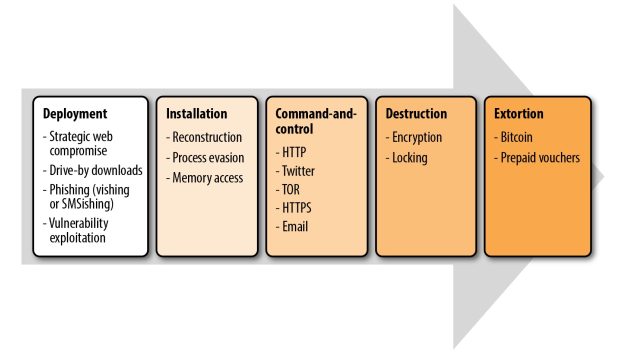
\includegraphics[width=\textwidth]{figuras/anatomy_of_a_ransomware_attack.png}
	\caption{Anatomy of a ransomware attack\cite{ransomware_oReilly}}
\end{figure}

\subsection{State of ransomware}
Ransomware is important for this project because it has gained much relevance in cybersecurity in the last years.
We think understanding it better is the first step to develop detection for it.
\linej
\linej
The main problems for studying ransomware is that is illegal and sometimes is hard to gather information.
For example most of the attacks are not reported and ransomware attacks are often analyzed offline and using auditing tools like decompilers because most of the time there is no source code\cite{ransomware_digital_extortion}.

\subsubsection{The growth of ransomware}
Next there are some estimations about the ransomware economy\cite{ransomware_economy}:
\begin{itemize}
	\item There are more than 6000 dark web marketplaces selling ransomware, with 45000 products listed.
	\item The ransomware marketplace on the dark web has grown in 2502\% from 2016 to 2017.
A major antimalware company states a 90\% increase in detection for business and a 93\% for individuals, in the same year\cite{ransomware_malwarebytes}.
	\item Some sellers of ransomware are making more than 100 thousand USD per year, just by retailing ransomware, when a legitimate software developer makes 30\% less.
\end{itemize}
\linej
Often ransomware includes remote control software to allow the remote execution of commands.
They often check if the server (certain ips or domains) can be reach before starting the process, waiting for a possible connection in the future if not.
Because these domain addresses are always resolving to new host ips, the criminal enterprises can regularly move around the Internet in relative safety, as they will always know their malcode can speak to them.
Keeping this Command and control server functional and anonymous may be hard and expensive depending on the approach used by the attacker.
They have evolved to use algorithms to generate a list of thousands of domains dynamically.
%Particularly DNS scans for new suspicious entries is advised.
\linej
The flaw of this approach is that can trigger behavioural alerts and reduces the scope of the attacks.
There is no need to initially contact the Command and control server, even for crypto ransomware because the public RSA key can be downloaded with the malware.
In some cases the attacker can command the malware to delete itself to avoid leaving evidence for security proffesionals\cite{ransomware_oReilly}\cite{ransomware_digital_extortion}.
\linej
\linej
The fundamental reason why this market exists is because the victims are willing to pay.
Is hard to know specifics because is estimated that most of the times these attacks are not reported (fewer are prosecuted and fewer are sentenced), but the mean crypto ransom is 300 USD per computer\cite{ransomware_digital_extortion}.
%\begin{figure}[H]
	%\centering
	%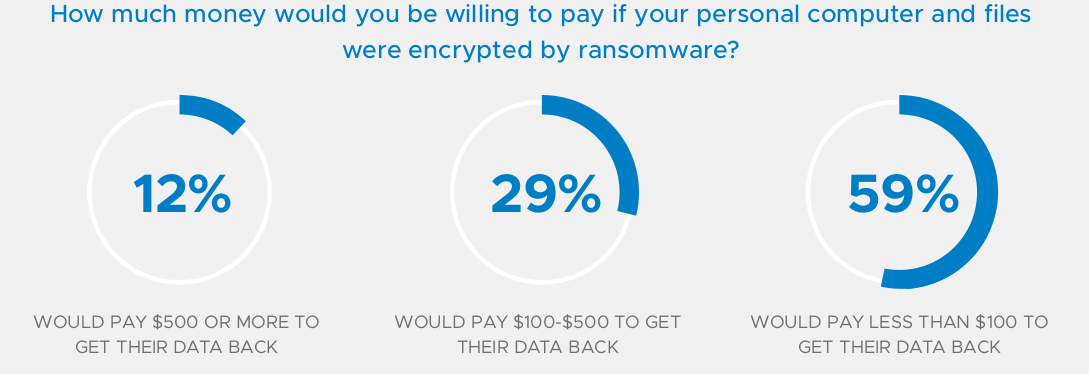
\includegraphics[width=\textwidth]{figuras/ransomware_pay_chance.png}
	%\caption{Statistics on the chance to pay ransomware\cite{ransomware_economy}}
%\end{figure}
\linej
\linej
Unlike many other forms of cyberattacks, ransomware can be quickly and brainlessly deployed with a high probability of profit nowadays.
It has been a revelant type of malware since its beginning 23 years ago, but in the last years its economy has grown hugely, mainly because\cite{ransomware_digital_extortion}\cite{ransomware_economy}:
\begin{itemize}
	\item Bitcoin and Tor: for pseudo-anonymous activities.
	\item Proliferation of service providers: anyone can get into the ransomware business because technical knowledge is not needed for every step of the process.
	\item Lack of fundamental security controls: such as backups, penetration testing, patching, etc.
\end{itemize}
\linej
Bitcoin allows money to be transferred in a way that makes it nearly impossible for law enforcement to follow the money trail.
Anyone can set up a free and unrestricted Bitcoin wallet address without needing any approval from financial institution, regulations, or dealing with providing evidence and proofs of identity, taxation, evidence of residence, and so on.
Anybody can see the Bitcoin transactions or the flow of the cryptocurrency from address to address in the blockchain, making it possible to backtrack it to a real identity.
Unfortunately cybercriminals use to mix transactions to make them very hard to follow, this is what Bitcoin mixing services are for.
\linej
Tor is an anonymity network, that can be used to mask illicit activities and can be used just by running a program.
\linej
Neither provides perfect anonymity, but both are very easy to use, which has lowered the risk and barrier to entry for ransomware perpetrators.
The requirement for ransoms to be paid over the Tor network has ensured there's no centralized endpoint to investigate with traditional geo-based law enforcement approaches\cite{ransomware_digital_extortion}.
\linej
\linej
Due to these innovations, the underground ransomware economy is now an industry that resembles commercial software. It can be divided into sections like: development, support, distribution and even help desks. This market can be divided into tiers\cite{ransomware_economy}:
\begin{itemize}
	\item Authors: They can be responsible for the creation of the malware (including frameworks) and training and support on them. In the current state of the market they can just remain as authors, without ever running the malware in other computers. The cost is based on how customized the code is for a particular target.
	\item RaaS: Ransomware-as-a-Service borrows from the Software-as-a-Service model. RaaS is designed to make ransomware available to even novice criminals. It provides technical and step-by-step information on how to launch the ransomware attack with the purchased software. The most sofisticated have a platform for checking the current status of the attack. In some cases the ransom is split among the members of the supply chain.
	\item Distributors: A high profit/risk tier. They can distribute it themselves by spam campaigns, social engineering, targeted hacks or exploit kits. They can also leverage RaaS.
\end{itemize}
\linej
Splitting the work into different modules makes the ransomware market more complex and competitive.
It encourages role specialization (increasing quality and reducing risk for authors), it makes it easier to enter (expanding the market) and the modularity increases the quantity of different products (making the malware change faster).
\linej
Of course making it easier to enter the market is a double edge sword, because it makes it easier for police to investigate.
Defenders have the inherent advantage of interrupting the entire attack if they can break or interrupt any link of the chain.
\linej
This market can be simplified into the next image:
\begin{figure}[H]
	\centering
	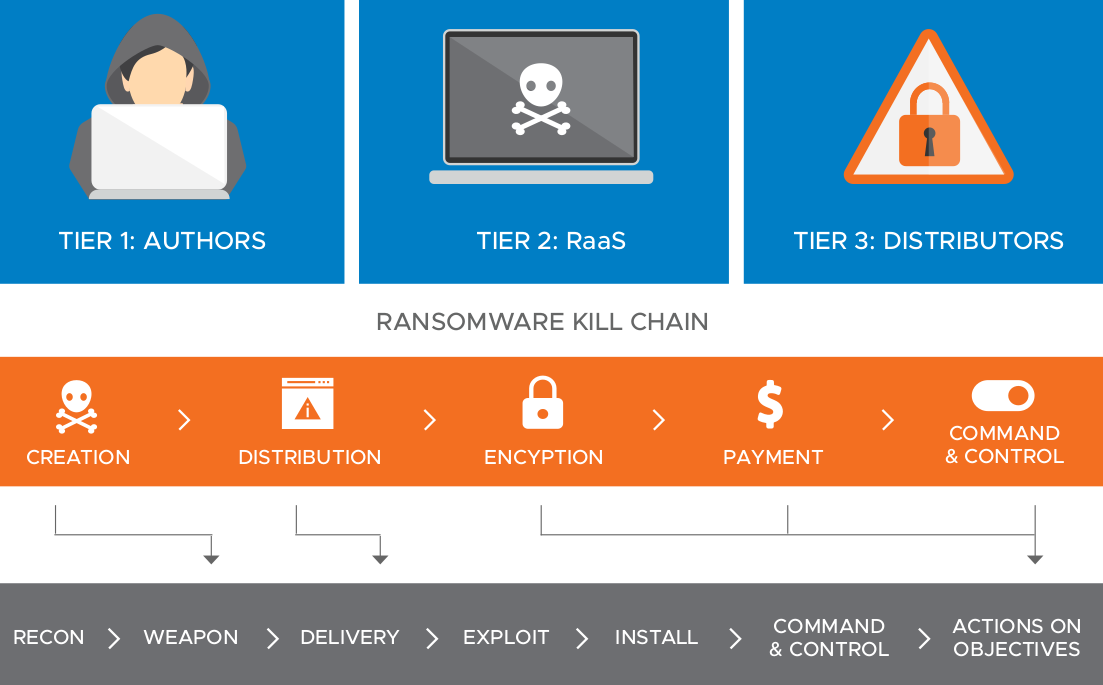
\includegraphics[width=\textwidth]{figuras/ransomware_chain.png}
	\caption{Ransomware supply chain and economy tiers\cite{ransomware_economy}}
\end{figure}
\linej
As long as the victims keep paying the ransom this trend will continue and the specialization will increase, resulting in more and bigger ransomware incidents.
%More creative forms of ransomware are sure to emerge over the years, like encrypting the master boot record\cite{ransomware_digital_extortion}.
The more ransomware is used the more secure the systems are against it, therefore in the future is also safe to assume that it would be more economical for criminals to use cryptominers or credential stealing instead\cite{ransomware_malwarebytes}.
\linej
\linej
Is also interesting to consider how ransomware and other attacks may take place if the main attack fails.
For example even if a ransomware attack fails it should be possible to use a distributed denial of service attack at greater cost and with lesser benefit.
A increase of malware as a distraction is expected in the future as the use and security of backups improves\cite{ransomware_economy}.

\subsubsection{Ransomware targets}
The more important the data the more money the victim is asked for.
Generally the bigger the business the better security it has and the more money cybercriminals can extort.
\linej
But the value of data may change from person to person, therefore there is no absolute best target for ransomware.
In the last years there has been an increase on the number of personal data sold in the dark web, which includes all kinds of data.
Cybercriminals can put pressure on the victim not only with direct ransom but also with the threat of selling the data.
\linej
In practice certain type of targets seems to rate higher on cybercriminals' priority lists\cite{ransomware_digital_extortion}:
\begin{enumerate}
	\item \textbf{Healthcare}: Apparently nothing sells as good on the black market as private healthcare records.
		Medical records do not lose value over time and they contain not only the person's medical history, but offers a full set of sensitive data that can be exploited in more ways than one (credit card numbers, social security numbers, banking credentials, e-mail IDs and employment history).
Cybercriminals use this currency to spread infections by phishing attacks, data fraud, and theft of medical histories.
	\item \textbf{Manufacturing}: Including businesses like automotive, electronics, textile and pharmacy.
The nature of the chemical and automotive businesses makes certain aspects horrifying, however, cybercriminals' motivation is predominantly financial, as they attack corporations not with the intention of mass murder, but to obtain valuable data and lucrative sensitive information.
	\item \textbf{Financial services}: The accessibility of payment methods and globally spread banking services whose main purpose is customer convenience will keep the financial industry high on the list. Attackers only need to impersonate or trick the victim in order to gain access to an account.
	\item \textbf{Goverment agencies}: They hold all types of personal and confidential data. If a goverment agency stops working it can affect many people.
	\item \textbf{Transportation}: Usually ransomware attacks set a time limit to pay the ransom, but in transportation real life sets the time limit. A higher effortless pressure results in less advance malware needs, meaning that transportation businesses could be effectively extorted with locker ransomware or denial of service attacks.
As in previous cases there is also interest in personal data and financial accounts.
	\item \textbf{Home users}: Ransomware is one of the best effective malware against personal computing users, who are considerably not experienced in cybersecurity.
This has increased due to the rise of smartphones and IoT devices.
Most users either don't use backups, they are not done often enough or they are stored in the same computer.
\end{enumerate}
\linej
In the end the target is always the people and the cybercriminal can either create a situation where is cheaper to pay or to gamble on the feelings (fear, shame, guilt, etc) of the victim.
\begin{figure}[H]
	\centering
	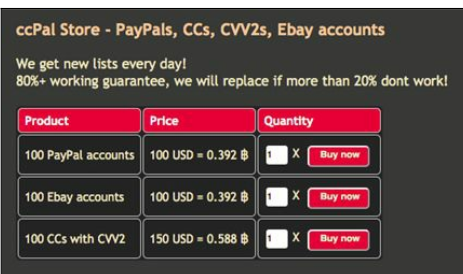
\includegraphics[width=.7\textwidth]{figuras/credit_cards_for_sale.png}
	\caption{Credit cards for sale\cite{ransomware_digital_extortion}}
\end{figure}

\subsection{Common patterns in crypto ransomware}
64\% of ransomware detected in 2016 was crypto ransomware\cite{ransomware_digital_extortion}, but it was not until 2013 that cybercriminals came back to it as their primary source of ransomware income\cite{ransomware_oReilly}.
The are many different crypto ransomware products, but we take interest in those who encrypt the files because, they are the ones that make the most impact on them.
If the encryption is done with strong algorithms it should not be possible to decrypt them in a lifetime (without knowing the decryption key).
\linej
\linej
This means suspicious activity regarding backups and files is common among the different crypto ransomware variants.
We assume the attacker prefers to execute the attack as fast as possible because:
\begin{itemize}
\item Once the encryption process starts is probably going to be detected very fast, either by an user or by an antimalware detector.
\item The only advantage of waiting is keeping the noise down.
\item If the encryption is only done on key files it should be very fast.
\item The system can be scanned quite silently before starting the encryption.
\end{itemize}
\linej
The most eficient way to encrypt the files is to use a symmetric algorithm (like AES-256), ensuring very strong and fast encryption even for big files.
The symmetric key is the same for encryption and decryption, and in this type of attack it holds the entire value of the ransom: once the ransom is paid the symmetric key is send to the victim to decrypt the files.
\linej
Obviously this key has to be kept secret by the attacker, therefore is ciphered with a public-key asymmetric algorithm (like RSA), allowing the attacker to transfer it without any risk.
Only the people with the private key should be able to decipher the symmetric key, therefore only the attacker can decipher it.
The public key is either downloaded with the malware or after the installation.
\linej
A major disadvantage of symmetric key encryption is that, in some cases, the key can be retrievered from RAM using special software.
Fortunately the DRAM in most systems is still live for anywhere from a few seconds to a few minutes after power loss, allowing a shutdown to stop the attack and still being able to recover from it.
However these techniques are unlikely to work with functions that avoid leaving trails in memory\cite{ransomware_oReilly}.

%\linej
%\linej
%Most ransomware families use the built-in Windows Crypto API to handle the encryption.
%While this is not a process that can necessarily be blocked, it is a process on which a security team can be alerted.
%The problem is not detecting its use, but rather not spawning false positives\cite{ransomware_oReilly}.

\subsubsection{File encryption and backup deletion}
This example shows how easily removal of local backups and encryption of files can be done with the right tools.
\linej
In this scenario the attacker uses AES for the files and ciphers the key passphrase with a RSA public key.
Both algorithms are supported by many tools: GnuGG, OpenSSL, custom DLLs and programming languages like PowerShell or Python.
OpenSSL was chosen because it works the same on Windows and GNU/Linux and is easy to use and install.
\linej
\linej
The first step would be the generation of the pair of RSA keys.
The private key stays in the computer of the attacker and the public key is stored into the victim's.
In this case the files are named ``keys.pem'' and ``public.pem'' respectively and the length of the key is 1024 bits.
The first file includes both private and public keys.
The second file is generated by the second command, which extracts the public key out of the combined file ``keys.pem''.
\begin{lstlisting}[style=PS,keywordstyle=\color{black}]
openssl genrsa -out keys.pem 1024
openssl rsa -in keys.pem -pubout -out public.pem
\end{lstlisting}
\linej
The next PowerShell script creates a random passphrase of letters, numbers and some special characters, which is used later for the symmetric key by the AES implementation of OpenSSL.
This passphrase is ciphered with the public RSA key and saved to the file ``passphrase.txt''.
Then script loops over all the files in \textit{C:/temp/} with the \textit{.ps1} extension, encrypting them to AES-256 (in block cipher mode) and deleting the original file when done.
The \textit{openssl} variable is just for convenience:
\lstinputlisting[style=PS]{src/ransomware_basic.ps1}
\linej
The passphrase file can be deciphered with the private key, getting the random passphrase used in the script:
\begin{lstlisting}[style=PS,keywordstyle=\color{black}]
openssl rsautl -decrypt -in passphrase.txt -inkey keys.pem
\end{lstlisting}
\linej
Decrypting the files can be done using the same passphrase, because AES is a symmetric algorithm.
This example assumes the same value for the variables as in the encryption process:
\lstinputlisting[style=PS]{src/ransomware_decrypt.ps1}
\linej
%TODO detection

\linej
\linej
Backups offer effective mitigation against crypto ransomware attacks in most cases.
There are many scenarios between distributed backups in servers accross the world and just having local backups.
Their ability to overcome ransomware attacks depends on multiple factors like: the exact malware, the distribution of the backup system, the security of the backup system, etc.
\linej
In this case we assume the target only has local backups that are managed with the Shadow Copy service, which allows files to be copied even when in use.
Some known ransomware like Locky and Cerber try to delete existing shadow copies before encrypting the files\cite{ransomware_oReilly}:
\begin{lstlisting}[style=PS]
C:\Windows\system32\vssadmin.exe delete shadows /all /quiet
C:\Windows\system32\wbem\wmic.exe shadowcopy delete
\end{lstlisting}
\linej
%TODO detection


%TODO Mitigation
%%MITIGATION
%%	Prevent the ransomware from accessing the Windows Registry
%%		Ransomware families use the registry to maintain persistence through reboots and to disable system restore on the victim machine.
%%		Administrators can disable writing to the registry, or at least to certain registry keys, using Windows Resource Protection.
%%	Cyber insurance
%%		in some cases
%%			costs like
%%				notifications costs to data breach victims
%%				legal defense costs
%%				forensics and investigation costs
%%	Decoy resources
%%	Security awareness and education
%%		particularly on e-mails and web browsing
%%		everyday documents: pdf, office macros
%%	Fundamental security controls
%%		backups, penetration testing, patching and software updates, firewall
%%	Restrictions to unnecessary services and software
%%		eg powershell or Tor
%%		for certain directories
%%		only allow digitally signed software
%%		deny access to vssadmin and wmic to avoid the deletion of shadowcopies
%%	Removing unused devices
%%		This action prevents possible further infection spreading and it should be applied to varied physical
%%		devices such as mapped drives, USB storage devices or memory sticks, smartphones, and cameras.
%%		All writeable devices should be removed from a station when not in use.
%%	File exchange management
%%		Businesses are based on sharing and it is impossible to do a job unless certain files are shared and
%%		worked on collaboratively. Once the process of file sharing becomes a routine, security gets on
%%		wobbly feet. To keep the filesystem safe, organizations should establish best practices for sharing
%%		data and files in a safe and secure manner. An effective way to minimize risks is application of digital
%%		signatures.
%%	Response plan development
%%		Prompt action is almost impossible if actors are unprepared. At a moment of crisis, decision-making
%%		can be weak and if the organization does not have an incident response plan at hand, the consequences
%%		of the infection can exacerbate. Developing a solid plan for fighting malware infections is the first
%%		mitigation task that should be completed by the responsible business leaders in the organization.
%%		A well-developed plan will prevent the company falling victim to payment at the moment of panic
%%		happening in the coal-and-ice a few hours after the attack.
%%		Several behaviors are key-avoiding payment and rather immediately referring to the incident plan,
%%		disconnecting infected units from the network, employing company digital security teams in line with
%%		the incident plan, keeping records of the information, and notifying law enforcement authorities.
%%
%%		Quick five-step guide for businesses under attack
%%			Disabling sync features:
%%				Enabled syncing features makes it easier for offenders to instigate
%%				attacks that will overwrite files, especially when they use crypto ransomware. By disabling sync
%%				features you can prevent targeting data in the cloud.
%%			Removing malware from the affected devices:
%%				Running a full scan is vital to remove the
%%				malware from the infected devices, including synced or mapped drives. Many operating systems
%%				come with a built-in basic anti-malware tool, which is not 100% effective. An advanced anti-
%%				malware software tool is the ultimate protective solution.
%%			File recovery:
%%				File recovery depends on the system version in use. For example, Windows
%%				users can recover files through the File Restore or System Protection functions.
%%			Blocking the payment transaction:
%%				Under certain circumstances, the payment transaction can
%%				be blocked, even if you have already started the payment process. This is throughble when the
%%				files have been successfully recovered without using the help provided by the attackers.
%%			Contacting law enforcement and reporting the crime:
%%				Getting in touch with the relevant
%%				cybercrime authority in the country is important not only for taking action in the concrete case,
%%				but also for predicting future criminal behavior and for undertaking protective measures to
%%				prevent similar attacks to other victims. Sending a report to the relevant software authorities is
%%				also recommended. By clicking the Send Report button you protect yourself and your
%%				organization, show solidarity, and contribute to a great business practice in building effective
%%				advanced anti-threat solutions.


%TODO Conclusion

